\section{Aufbau}
Der physische Aufbau des verwendeten Billardtisches, der Kamera und des Projektors wurden aus der Vorarbeit \cite{project2:aufbau} übernommen.
Nachfolgend werden die wichtigsten Informationen wiederholt.

Die Kamera wie auch der Projektor wurden mithilfe eines Baugerüsts über dem Tisch platziert.
Dieses ermöglicht die nötige Flexibilität, um die Geräte unabhängig voneinander optimal auszurichten.
Der Aufbau ist in Abbildung \ref{fig:construction} ersichtlich.

\begin{figure}[h!]
    \begin{center}
        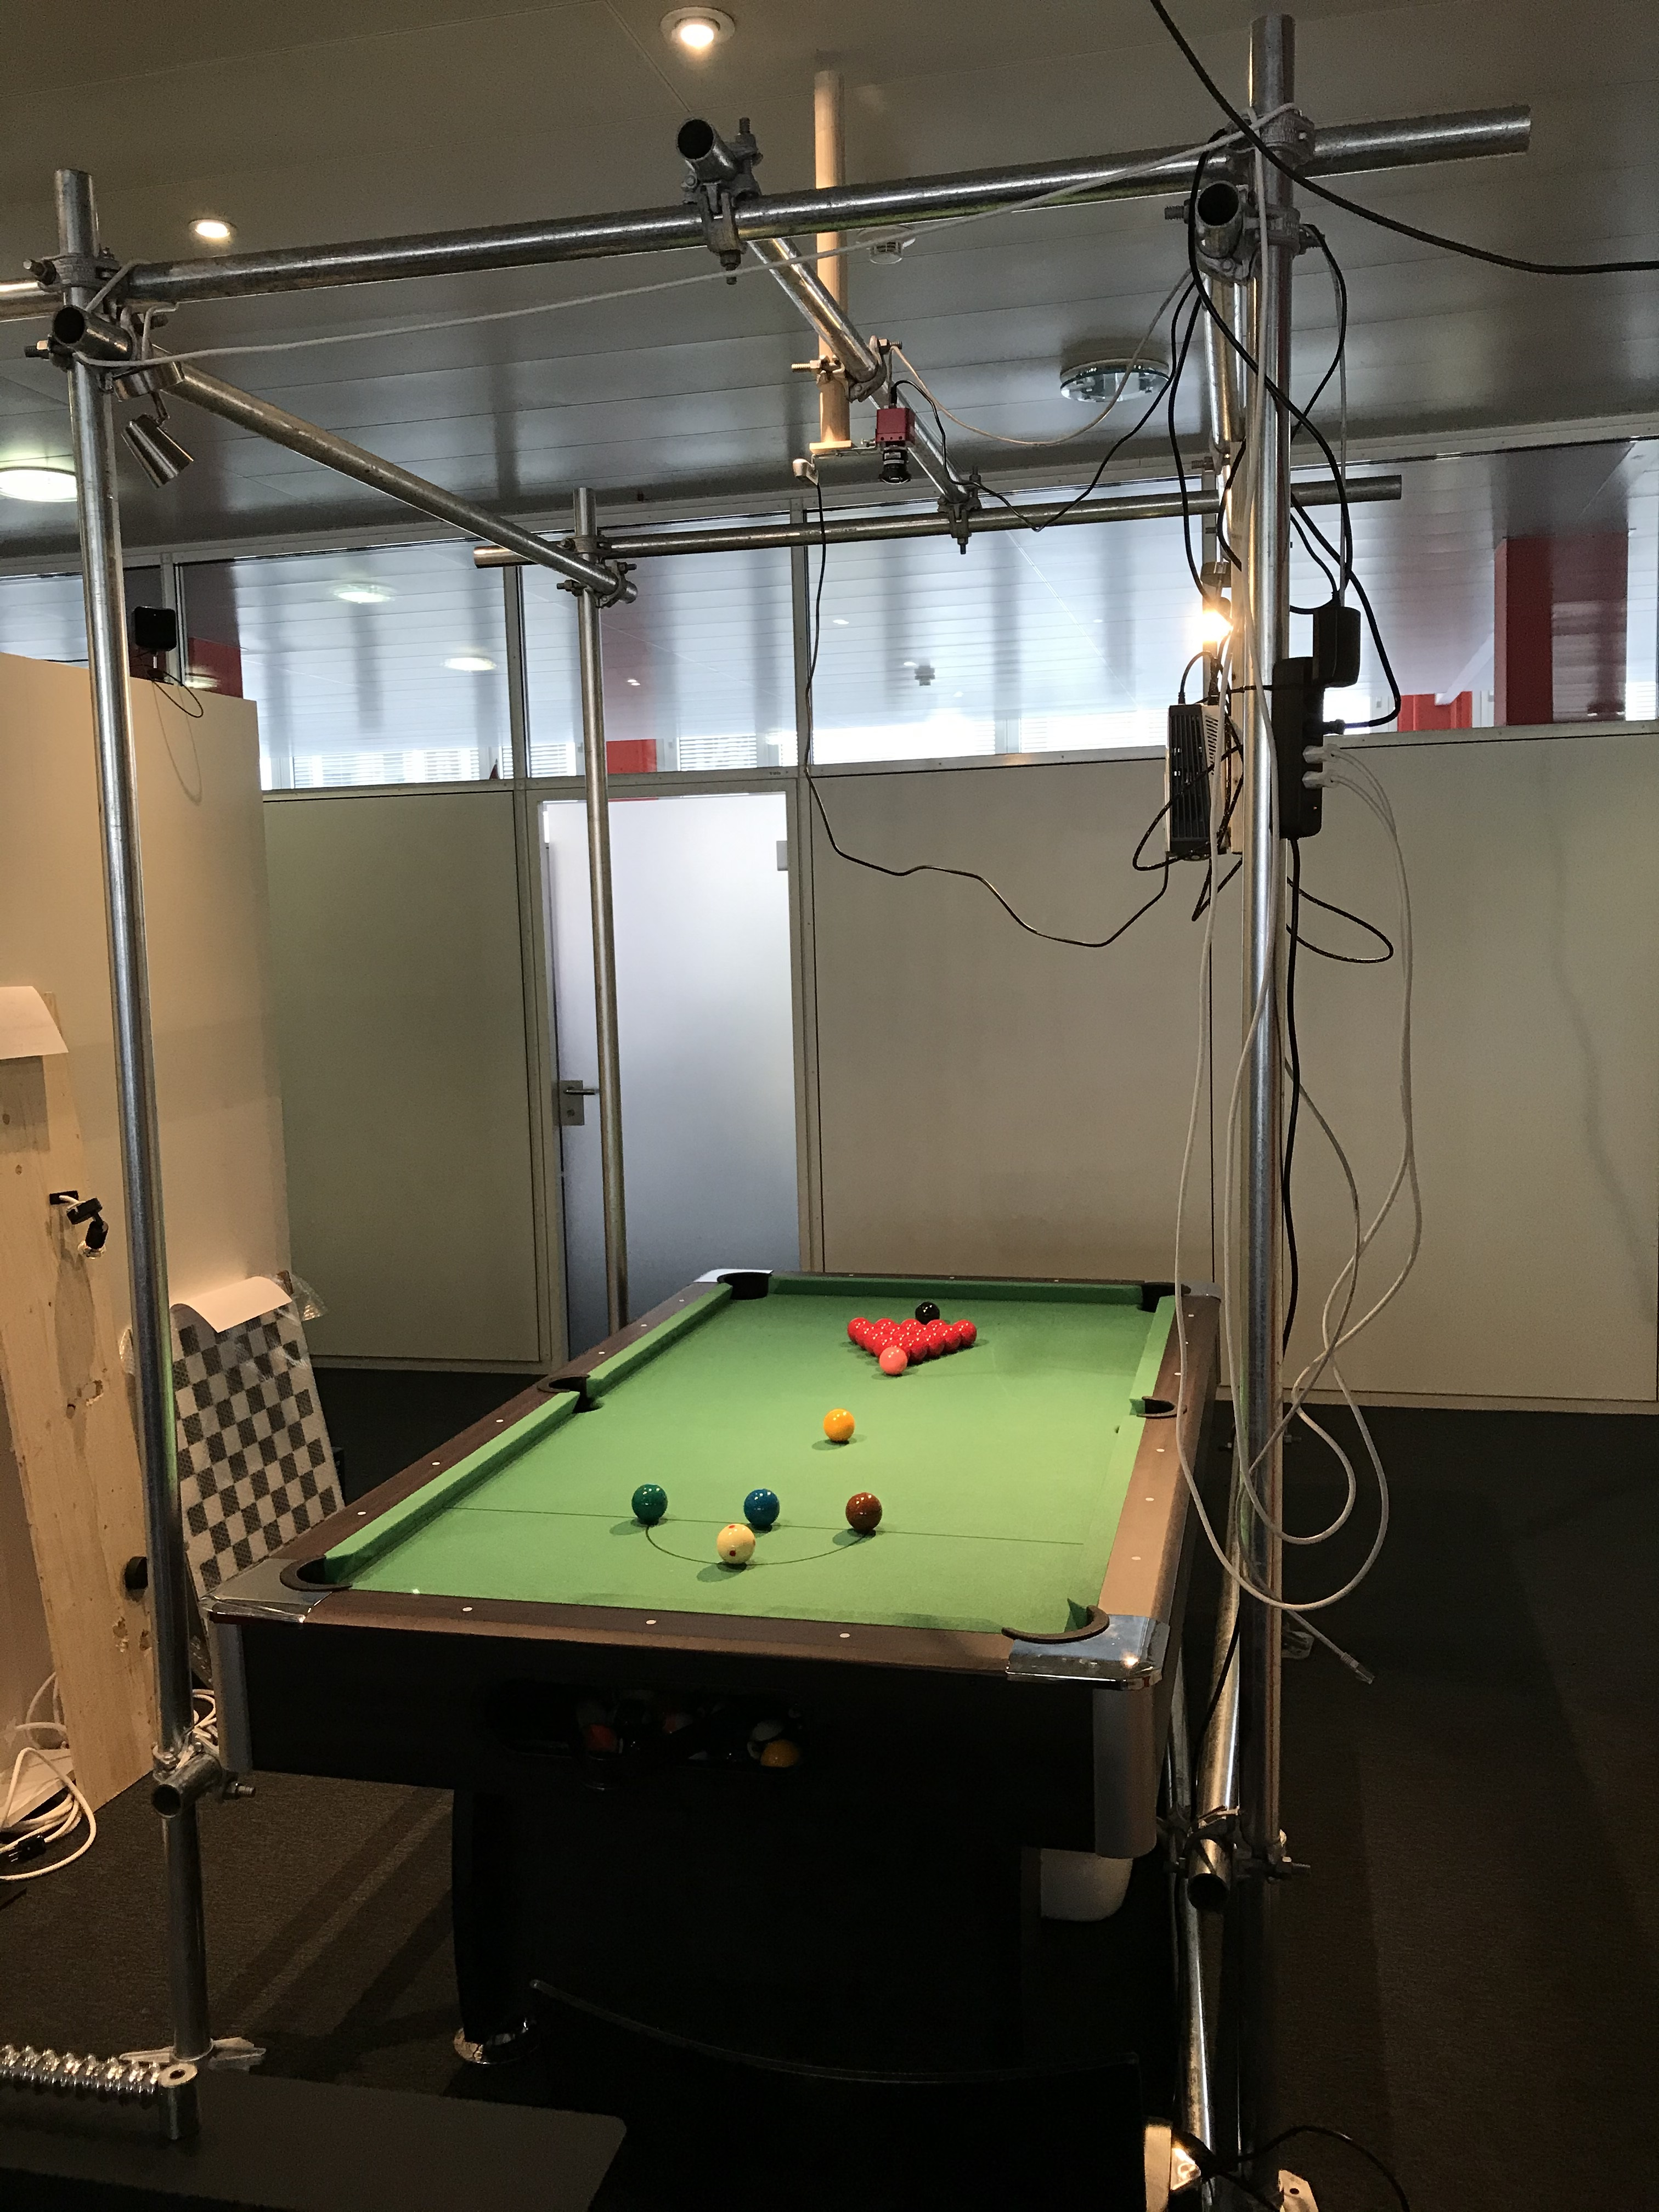
\includegraphics[width=0.6\linewidth]{../common/03_billiard_ai/resources/table.jpg}
    \end{center}
    \caption{Baugerüst mit montierter Kamera und Beamer \cite{project2:aufbau}.}
    \label{fig:construction}
\end{figure}

\subsection{Kamera}\label{kap:camera}

Als Kamera wurde eine Intel RealSense Depth Camera D435 verwendet \cite{intel:realsense_d435}.
Die intrinsischen Kameraparameter des Farbsensors wurden mithilfe des RealSense SDK 2.43.0 \cite{github:realsense_sdk} ausgelesen.
Beim Farbsensor handelt es sich um einen \emph{OmniVision OV2740} \cite{intel:realsense_d435_datasheet}.
Die Auflösungs des Sensors beträgt 1920x1080 und die Pixelgrösse beträgt \SI{1.4}{\micro\metre} \cite{omnivision:ov2740}.

Nachfolgend ist die allgemeine intrinsische Kameramatrix in \emph{column-major order} aufgeführt.
Siehe \cite{matlab:what_is_camera_calibration} für die Erläuterung der Parameter in \emph{row-major order}.

\begin{align}
    \begin{pmatrix}
        f_x & s   & c_x\\
        0   & f_y & c_y\\
        0   & 0   & 1
    \end{pmatrix}
\end{align}

Die konkreten Werte für die Brennweite $(f_x, f_y)$ [Pixel], das optische Zentrum $(c_x, c_y)$ [Pixel]
und der Schiefekoeffizient $s$ sind nachfolgend eingefügt.

\begin{equation}
    \begin{pmatrix}
        1375.68884 & 0          & 974.842407\\
        0          & 1375.85425 & 539.362732\\
        0          & 0          & 1
    \end{pmatrix}
\end{equation}

Die Parameter für die Modellierung der radialen und tangentialen Verzerrung $k_1$, $k_2$, $k_3$, $p_1$, $p_2$ sind gemäss
RealSense SDK alle 0 und das verwendete Modell wird \emph{Inverse Brown-Conrady} genannt.

\subsection{Projektor}\label{kap:projector}

Der eingesetzte Projektor ist ein \emph{BenQ MW820ST}, siehe \cite{projectorcentral:benq_mw820st}.
Es handelt sich um einen Kurzdistanzbeamer, welcher etwa 1\si{\metre} über dem Billiardtisch angebracht wurde.
